
\begin{titlepage}
    \begin{table}[H]
        \centering
        \setlength{\arrayrulewidth}{1pt}  % Adjusts the thickness of the borders
        \arrayrulecolor{black}            % Sets the color of the borders to black
        \renewcommand{\arraystretch}{1}   % Reset any existing row stretch settings
        \begin{tabularx}{\textwidth}{|>{\centering\arraybackslash}X|>{\centering\arraybackslash}X|>{\centering\arraybackslash}X|}
            \hline
            % Insert in first colum the logo of the company
            \multicolumn{3}{|c|}{
\includegraphics[width=0.4\textwidth]{ressources-graphiques/logos/logo_simonin.png}} \\  % Second row with height set to 3 cm
            \hline
            \hline
            \multicolumn{3}{|c|}{\rule{0pt}{1cm}\fontsize{26}{40}\selectfont DESCENTE DE CHARGES  }        \\  % First row with height set to 3 cm
            \hline
            \hline
            {
\includegraphics[width=0.3\textwidth]{input_data/maitrise_ouvrage.png}} &
            {
\includegraphics[width=0.3\textwidth]{input_data/architectes.png}} &
            {
\includegraphics[width=0.3\textwidth]{input_data/bureau_etudes_controle.png}} \\
            \hline
            \hline
            \multicolumn{2}{|c|}{\rule{0pt}{3cm}\fontsize{16}{40}\selectfont \titreprojet} & \multirow{3}{*}{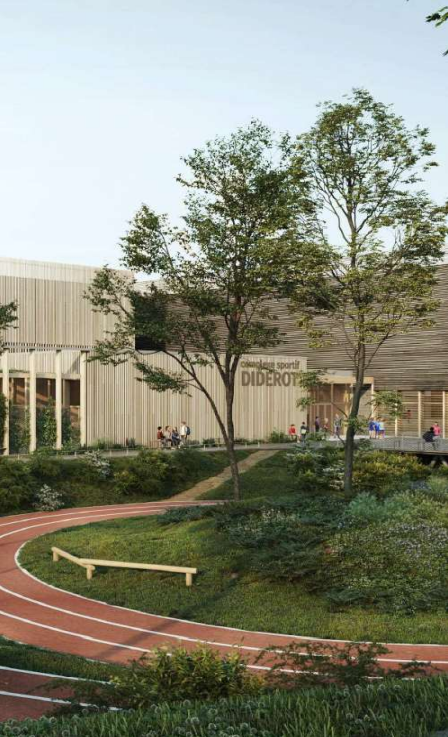
\includegraphics[width=\linewidth, width=3cm, keepaspectratio]{input_data/image_projet_page_de_garde.png}} \\
            \multicolumn{2}{|c|}{\rule{0pt}{3cm}\fontsize{16}{40}\selectfont \soustitreprojet} & \\
            \multicolumn{2}{|c|}{\rule{0pt}{3cm}\fontsize{16}{40}\selectfont} & \\
            \hline
            \hline
        % \label{tab:fullwidth}
        \end{tabularx}
   \end{table}
    
   
    % Table of Modifications
    \centering
    \begin{tabularx}{\textwidth}{|l|l|X|l|l|}
        \hline
        \textbf{Date}   & \textbf{Index} & \textbf{Modifications}        & Rédacteur:       & {\redacteur}           \\ \hline
        XXXX-XX-XX      & 1              & Création du document          &                  & {\emailredacteur}      \\ \hline
                        &                &                               & Vérificateur     & {\verificateur}        \\ \hline
                        &                &                               &                  & {\emailverificateur}    \\ \hline
                        &                &                               & Affaire N°:      & {\numeroaffaire}    \\ \hline
                        &                &                               & Réf.S :          & {\numeroreference}  \\ \hline
                        &                &                               & \textbf{Doc N°:} & \textbf{\numerodoc} \\ \hline
    \end{tabularx}


    % {\large \today\par} % Date en bas de page


\end{titlepage}





% \begin{titlepage}
%     \thispagestyle{empty}

%     \input{packages/overlay_STB.tikz}

%     % L'intitulé du stage
%     \begin{textblock*}{12cm}(4.5cm,2.5cm)
%         \begin{LARGE}
%             \makeatletter
%             \justifying
%             \begin{center}
%                 \textbf{\textcolor{white}{\jobposition}}
%                 \\
%                 \textbf{\textcolor{white}{\thetitle}}
%             \end{center}
%             \makeatother
%         \end{LARGE}
%     \end{textblock*}

%     % Nom Prénom
%     \begin{textblock*}{10cm}(2.5cm, 7.5cm)
%         \raggedright
%         \large
%         \textbf{\textcolor{white}{NOM Prénom}}
%         \\
%         \textbf{\textcolor{white}{\theauthor}}
%     \end{textblock*}

%     % Responsable Pédagogique
%     \begin{textblock*}{10cm}(2.5cm, 9.5cm)
%         \raggedright
%         \large
%         \textbf{\textcolor{white}{Responsable Pédagogique}}
%         \\
%         \textbf{\textcolor{white}{\theRPeda}}
%     \end{textblock*}


%     % Branche
%     \begin{textblock*}{10cm}(12cm,7.5cm)
%         \raggedright
%         \large
%         \textbf{\textcolor{white}{Branche}}
%         \\
%         \begin{raggedleft}
%             \textcolor{white}{\theUE}
%         \end{raggedleft}
%     \end{textblock*}

%     % Semestre
%     \begin{textblock*}{10cm}(12cm,9.5cm)
%         \large
%         \raggedright
%         \textbf{\textcolor{white}{Année}}
%         \\
%         \textcolor{white}{\theSemestre}
%     \end{textblock*}

%     % Titre du résumé du stage
%     \begin{textblock*}{18cm}(1.5cm,11cm)
%         \begin{center}
%             \normalsize
%             \textbf{\textcolor{bleuRoiUTT}{Résumé (150 mots)}}
%         \end{center}
%     \end{textblock*}

%     % Résumé du stage
%     \begin{textblock*}{16cm}(2.54cm,13cm)
%         {
%             \normalsize
%             \makeatletter
%             \setlength{\parindent}{0pt}
%             \titletext
%         }
%     \end{textblock*}

%     % Mots clés (Thésaurus)
%     \begin{textblock*}{9cm}(10cm,21.75cm)
%         \normalsize
%         \centering
%         \textbf{\textcolor{white}{Mots clés (cf Thésaurus)}}
%     \end{textblock*}

%     \begin{textblock*}{10cm}(9.5cm,21.75cm)
%         \small
%         \textcolor{white}{
%             \begin{itemize}[label=\textcolor{white}{\textbullet}]
%                 \item \textbf{\theKone}
%                 \item \textbf{\theKtwo}
%                 \item \textbf{\theKthree}
%                 \item \textbf{\theKfourth}
%             \end{itemize}
%         }
%     \end{textblock*}

%     % Entreprise / Lieu / Responsable
%     \begin{textblock*}{6.5cm}(2.5cm,21cm)
%         \small
%         \raggedright
%         \justify
%         \textbf{\textcolor{bleuRoiUTT}{Entreprise :} \theEntreprise}
%     \end{textblock*}

%     \begin{textblock*}{6.5cm}(2.5cm,22cm)
%         \small
%         \raggedright
%         \justify
%         \textbf{\textcolor{bleuRoiUTT}{Lieu :} \textit{\mapAddr{\theLieu}}}
%     \end{textblock*}

%     \begin{textblock*}{6.5cm}(2.5cm, 23cm)
%         \small
%         \raggedright
%         \justify
%         \textbf{\textcolor{bleuRoiUTT}{Responsable :} \theREntre}
%     \end{textblock*}

% \end{titlepage}

% \clearpage % flushes out all floats that have been deferred